\newcommand{\files}[1]{
    \hfill
    \mbox{
        $\hookrightarrow$
        \texttt{#1}
    }
}

\section{Lautsprecher}
\label{sec:1}
\blindtext

\def\arraystretch{1.3}
\begin{table}[h]
    \centering
    \caption{Eine Tabelle}
    \label{tab:mics}
    \begin{tabular}{l l l l l}
        Hersteller & Typ & Akustische Arbeitsweise & Richtcharakteristik & Einfallsrichtung \\
        \hline
        Shure & \texttt{SM58} & Druckgradienten-/Schnelleempfänger & Niere & 0°, 90°, 180° \\
    \end{tabular}
\end{table}


\subsection{Abstrahlcharakteristik}
\label{subsec:a}
Abbildung \ref{fig:balloon} zeigt die Abstrahlcharakteristik eines Cellos bei verschiedenen Frequenzen in Oktavabstand.
Für eine anschauliche Darstellung wurden die Werte normiert, sodass der niedrigste Wert auf 20 dB liegt.
Mit steigender Frequenz ist zu erkennen, dass die Schalldruckpegelwerte im allgemeinem abnehmen.
Darüber hinaus deformiert sich die zunächst sphärische Form des Ballons zu den hohen Frequenzen hin mit hervortretenden Beulen.

\begin{figure}[bth]
    \centering
    \begin{subfigure}{.5\textwidth}
        \centering
        \caption{125 Hz}
        \includegraphics[width=0.85\linewidth]{Figures/125Hz.eps}
    \end{subfigure}%
    \begin{subfigure}{.5\textwidth}
        \centering
        \caption{250 Hz}
        \includegraphics[width=0.85\linewidth]{Figures/250Hz.eps}
    \end{subfigure}

    \begin{subfigure}{.5\textwidth}
        \centering
        \caption{500 Hz}
        \includegraphics[width=0.85\linewidth]{Figures/500Hz.eps}
    \end{subfigure}%
    \begin{subfigure}{.5\textwidth}
        \centering
        \caption{1000 Hz}
        \includegraphics[width=0.85\linewidth]{Figures/1000Hz.eps}
    \end{subfigure}

    \begin{subfigure}{.5\textwidth}
        \centering
        \caption{2000 Hz}
        \includegraphics[width=0.85\linewidth]{Figures/2000Hz.eps}
    \end{subfigure}%
    \begin{subfigure}{.5\textwidth}
        \centering
        \caption{4000 Hz}
        \includegraphics[width=0.85\linewidth]{Figures/4000Hz.eps}
    \end{subfigure}

    \begin{subfigure}{.5\textwidth}
        \centering
        \caption{8000 Hz}
        \includegraphics[width=0.85\linewidth]{Figures/8000Hz.eps}
    \end{subfigure}

    \caption{Abstrahlcharakteristik eines Cellos bei verschiedenen Frequenzen in Oktavabstand}
    \label{fig:balloon}
\end{figure}


\subsection{Frequenzgang}
\label{subsec:b}
\blindtext


\subsection{Untersektion}
\label{subsec:c}

\begin{figure}[bth]
    \centering
    \begin{subfigure}{.49\textwidth}
        \centering
        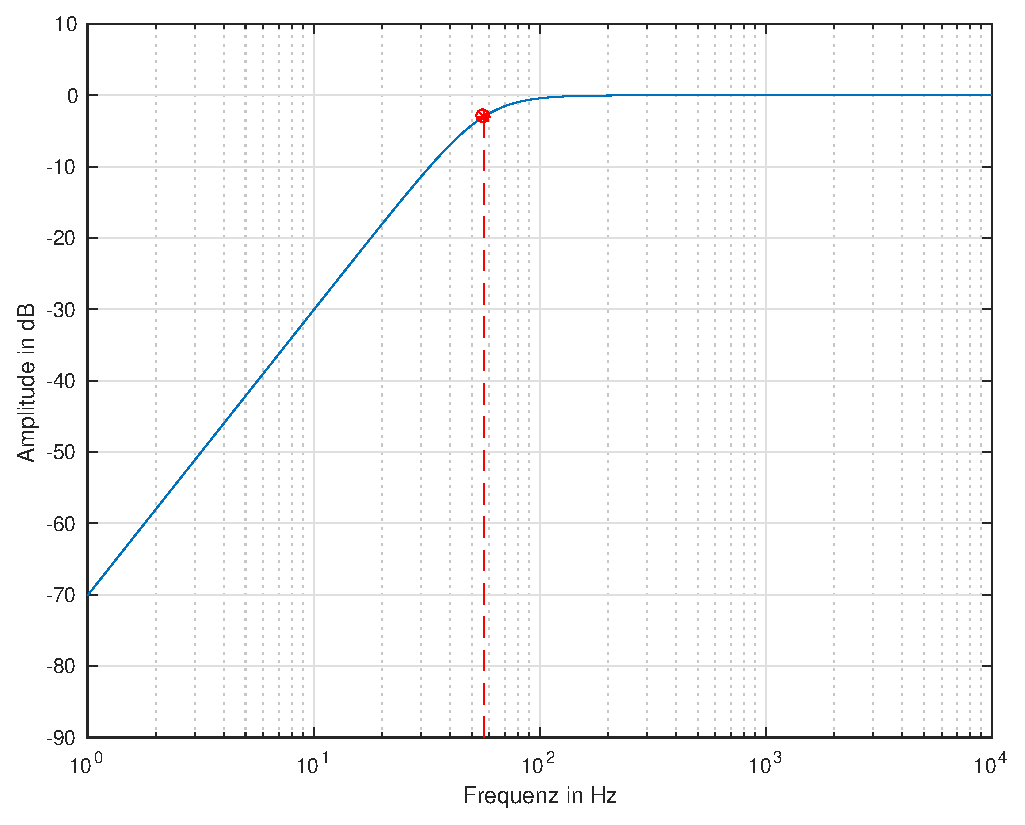
\includegraphics[width=0.85\linewidth]{Figures/Normaler_Frequenzgang.eps}
        \caption{Normaler Frequenzgang}
        \label{Normaler_Frequenzgang}
    \end{subfigure} 
    \begin{subfigure}{.49\textwidth}
        \centering
        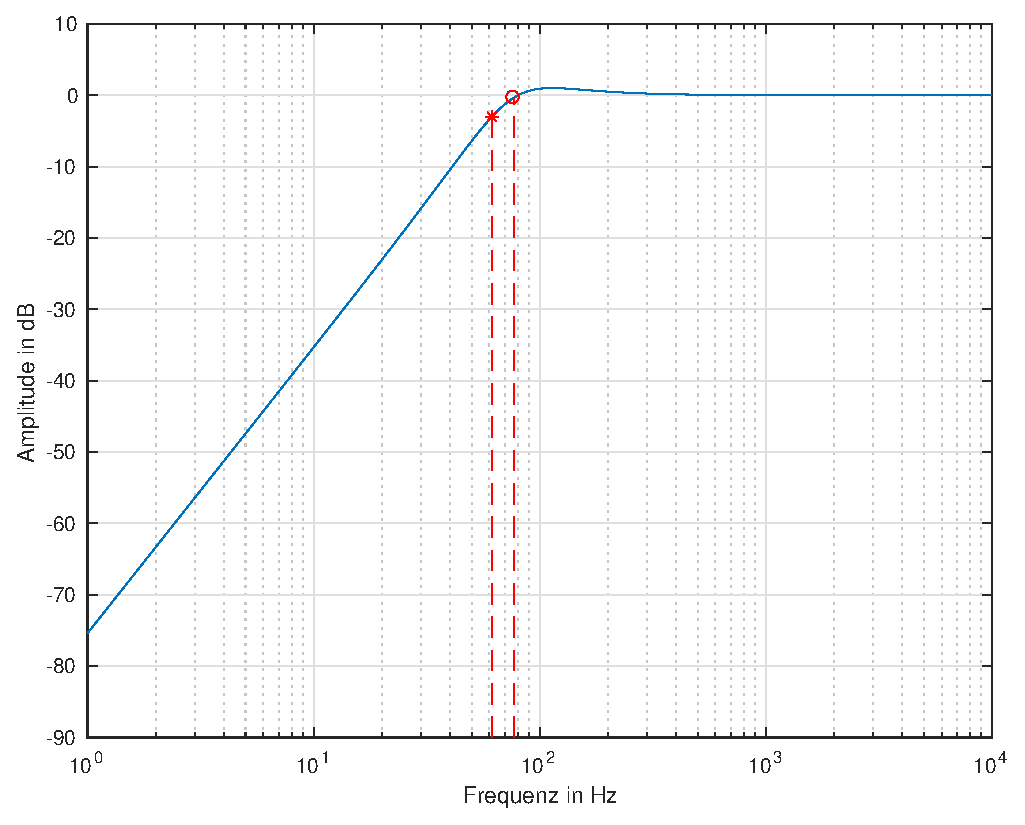
\includegraphics[width=0.85\linewidth]{Figures/Frequenzgang_1dB.eps}
        \caption{Frequenzgang bei 1dB Überhöhung}
        \label{Frequenzgang_1dB}
    \end{subfigure}

    \begin{subfigure}{.5\textwidth}
        \centering
        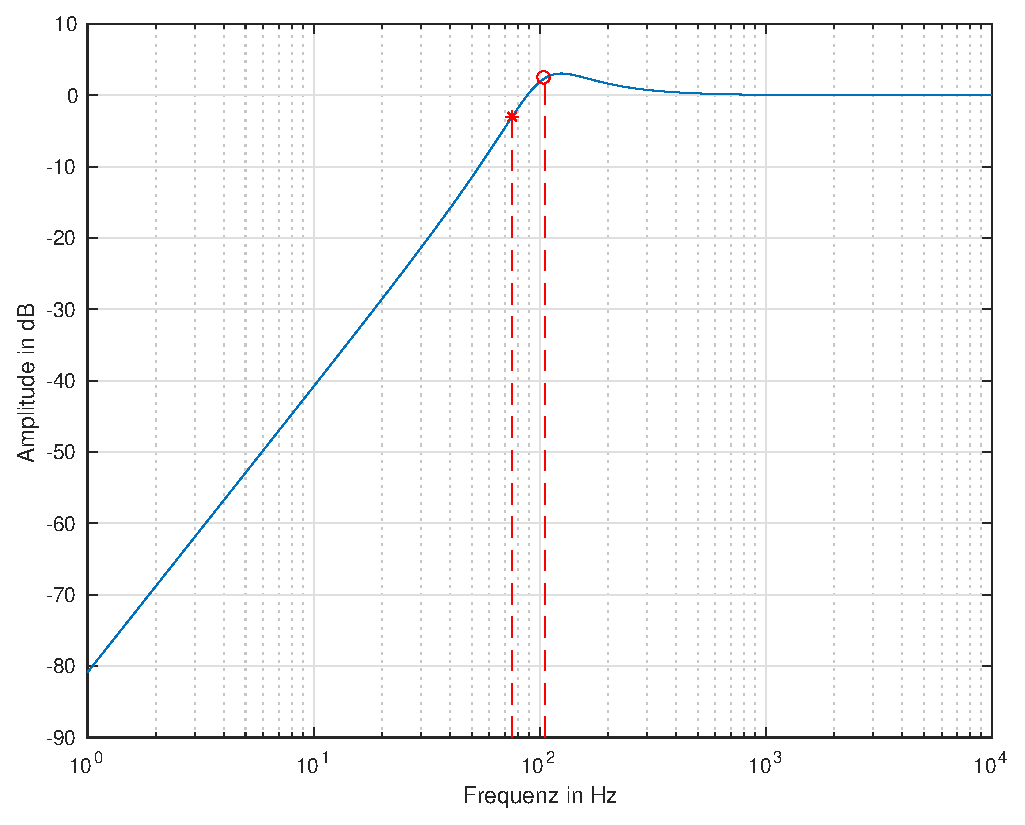
\includegraphics[width=0.85\linewidth]{Figures/Frequenzgang_3dB.eps}
        \caption{Frequenzgang bei 3dB Überhöhung}
        \label{Frequenzgang_3dB}
    \end{subfigure}
\end{figure}